%iffalse
\let\negmedspace\undefined
\let\negthickspace\undefined
\documentclass[journal,12pt,onecolumn]{IEEEtran}
\usepackage{cite}
\usepackage{amsmath,amssymb,amsfonts,amsthm}
\usepackage{algorithmic}
\usepackage{graphicx}
\usepackage{textcomp}
\usepackage{xcolor}
\usepackage{txfonts}
\usepackage{listings}
\usepackage{enumitem}
\usepackage{mathtools}
\usepackage{gensymb}
\usepackage{comment}
\usepackage[breaklinks=true]{hyperref}
\usepackage{tkz-euclide} 
\usepackage{listings}
\usepackage{gvv}                                        
%\def\inputGnumericTable{}                                 
\usepackage[latin1]{inputenc}                                
\usepackage{color}                                            
\usepackage{array}                                            
\usepackage{longtable}                                       
\usepackage{calc}                                             
\usepackage{multirow}                                         
\usepackage{hhline}                                           
\usepackage{ifthen}                                           
\usepackage{lscape}
\usepackage{tabularx}
\usepackage{array}
\usepackage{float}
\usepackage{pgfplots}


\newtheorem{theorem}{Theorem}[section]
\newtheorem{problem}{Problem}
\newtheorem{proposition}{Proposition}[section]
\newtheorem{lemma}{Lemma}[section]
\newtheorem{corollary}[theorem]{Corollary}
\newtheorem{example}{Example}[section]
\newtheorem{definition}[problem]{Definition}
\newcommand{\BEQA}{\begin{eqnarray}}
\newcommand{\EEQA}{\end{eqnarray}}
\newcommand{\define}{\stackrel{\triangle}{=}}
\theoremstyle{remark}
\newtheorem{rem}{Remark}

% Marks the beginning of the document
\begin{document}
\bibliographystyle{IEEEtran}
\vspace{3cm}

\title{assignment2:1.5.4}
\author{AI24BTECH11007 - Sri Sathwik Desaboina}
\maketitle
\bigskip

\renewcommand{\thefigure}{\theenumi}
\renewcommand{\thetable}{\theenumi}
\textbf{Question}:\\
A circle has its center at $\myvec{4\\4}$. If one end of a is $\myvec{4\\0}$, then find the coordinates of the other end.
\\
\textbf{Solution: }
\begin{table}[h!]    
    \centering
    \begin{tabular}[12pt]{ |c| c| c|}
    \hline
    \textbf{S.No} & \textbf{variables used}&\textbf{description}\\ 
    \hline
	$1$ & \textit{t} & a variable which takes the real values in the range $(-1,1)$\\
    \hline
	$2$ & \textit{a} & it is a fixed real number \\
    \hline
	$3$ & $\vec{A(t)}$ & it is a transformation matrix of parameter t\\
    \hline
	$4$ & $\vec{v(t)}$ & it represent the parameter t and allows to define x and y \\
    \hline
	$5$ & $\vec{p(t)}$ & a point with coordinates x and y. \\
    \hline
    \end{tabular}

    \caption{Input parameters }
    \label{table}
  \end{table}
Since the centre $\vec O$ is the mid point of $\vec A$ and $\vec B$.

\begin{align}
	\vec O &= \myvec{\frac{x_1+4}{2}\\\frac{y_1+0}{2}} \\
	\myvec{\frac{x_1 + 4}{2}\\\frac{y_1 + 0}{2}} &= \myvec{4\\4} \\
	\frac{x_1 + 4}{2} &= 4 \implies
	x_1 = 4 \\
	\frac{y_1 + 0}{2} &= 4 \implies
	y_1 = 8
\end{align}

$\therefore$ $\vec B\myvec{x_1\\y_1}$=$\vec B\myvec{4\\8}$.






 Plot:

\begin{figure}[h!]
    \centering
	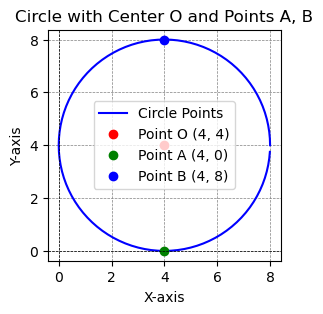
\includegraphics[scale=1]{figs/circle_plot.png}
	\caption{Circle with center $\myvec{4\\4}$ and diameter points A$\myvec{4\\0}$ and B$\myvec{4\\8}$.}
    \label{fig:circle_plot}
\end{figure}


\end{document}









